Sha-3 ist eine vom US-amerikanischen "National Institute of Standards and Technology" definierte Familie von kryptographischen Hashfunktion.
Dazu wird die Eingabe mithilfe eines \textbf{Paddings} in mehere gleich große Blöcke aufgeteilt. Die Blöcke werden nacheinander über eine \textbf{Schwammkonstruktion}
zu einem 1600 Bit breiten Bitvektor kombiniert, woraus dann der endgültige Hash ausgelesen wird. 

\newcommand{\bigcomp}{%
  \DOTSB
  \mathop{\vphantom{\sum}\mathpalette\bigcomp@\relax}%
  \slimits@
}
\newcommand{\bigcomp@}[2]{%
  \begingroup\m@th
  \sbox\z@{$#1\sum$}%
  \setlength{\unitlength}{0.9\dimexpr\ht\z@+\dp\z@}%
  \vcenter{\hbox{%
    \begin{picture}(1,1)
    \bigcomp@linethickness{#1}
    \put(0.5,0.5){\circle{1}}
    \end{picture}%
  }}%
  \endgroup
}
\newcommand{\bigcomp@linethickness}[1]{%
  \linethickness{%
      \ifx#1\displaystyle 2\fontdimen8\textfont\else
      \ifx#1\textstyle 1.65\fontdimen8\textfont\else
      \ifx#1\scriptstyle 1.65\fontdimen8\scriptfont\else
      1.65\fontdimen8\scriptscriptfont\fi\fi\fi 3
  }%
}

\section{Keccak-Permutation}
Als Grundlage für SHA-3 dient eine Instanz der Keccak-Permutationsfamilie KECCAK-f.
Für eine kryptographische Sicherheitsanalyse betrachtet man in der Regel das asymptotische Verhalten der erwarteten Laufzeit eines Angreifers.
Hierzu benötigt man eine Funktion mit variablem Sicherheitsparameter, damit diese Analyse durchgeführt werden kann.
Wir interessieren uns hier allerdings nur für die konkrete Instanz mit einem festen Sicherheitsparameter, die vom SHA-3 Standard[Cite missing] festgelegt wird, genauer für $SHA3-256$.
Die genaue Definition mit variablem Sicherheitsparameter ist zum Nachlesen auch in [Cite missing] angegeben.
Wir wollen uns nun zuerst einmal den Zustandsvektor ein wenig genauer anschauen, bevor wir uns die fünf Unterfunktionen ansehen, aus denen die KECCAK-f Permutation aufgebaut ist.

\subsection{Zustandsvektor}
Die KECCAK-f Permutation arbeitet auf einem 1600 Bit breiten Zustandsvektor, auch \textbf{State Array} genannt.
Am besten lässt er sich als dreidimensionale Struktur der Form 5x5x64 Bit vorstellen, siehe Abb. \ref{fig:statearray}.

\begin{figure}
	\center
	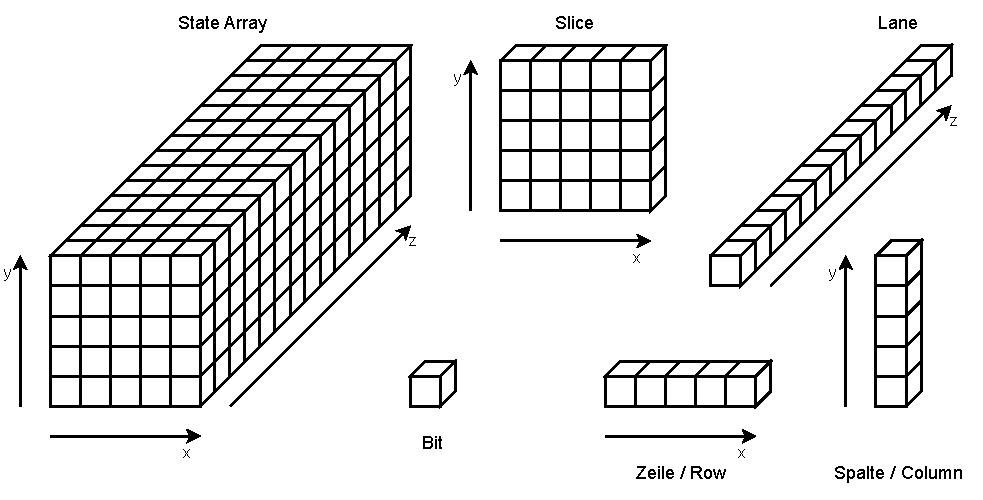
\includegraphics{images/StateArrayBeschreibung.pdf}
	\caption{Blockrepräsentation des State Array}
	\label{fig:statearray}
\end{figure}

Die Konvertierung eines eindimensionalen Vektors \textbf{V} in dieses dreidimensionale State Array \textbf{A} funktioniert wie folgt:
\begin{align*}
	\textbf{A}[x][y][z] \coloneq \textbf{V}[64(5y + x) + z] & \forall x,y = 0,...,4; z = 0,...,63
\end{align*}
Die Lanes werden also der Reihe nach erst in x-Richtung und dann in y-Richtung mit dem Inhalt von \textbf{V} gefüllt.

\subsection{Konventionen}
\begin{align*}
    \textbf{A},\ \textbf{A}^\prime & : \text{ State Array}, \\
    \textbf{B},\ \textbf{C} & : \text{ Ein Vektor aus 5 Lanes (von 0 bis 4)}, \\
    r & : \text{ Ein Rundenindex (von 0 bis 23)}
\end{align*}

\subsection{Theta-Unterfunktion}
\begin{figure}
    \center
    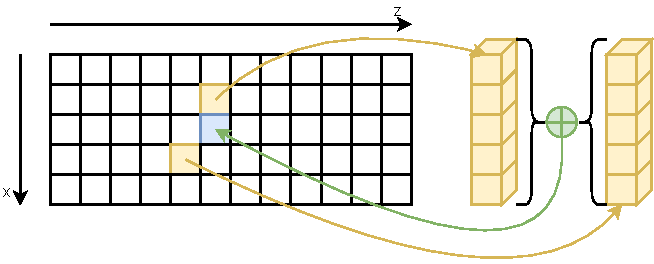
\includegraphics{images/theta.pdf}
    \caption{Spaltensummierung der $\theta$-Funktion}
    \label{fig:definition_theta}
\end{figure}
Die erste Unterfunktion der Keccak-Permutation ist Theta ($\theta$). Sie modifiziert jedes Bit eines State Arrays, indem sie zwei benachbarte Spalten auf das Bit aufsummiert, siehe Abb. \ref{fig:definition_theta}.
\begin{align*}
    \theta (\textbf{A}) & \coloneq \textbf{A}^\prime \text{ mit } \\
    \textbf{C}[x] & \coloneq \textbf{A}[x][0] \oplus ... \oplus \textbf{A}[x][4] && \forall x = 0,...,4 \\
    \textbf{D}[x] & \coloneq \textbf{C}[(x - 1) mod\ 5] \oplus rotr(C[(x + 1) mod\ 5], 1)\ && \forall x = 0,...,4 \\
    \textbf{A}^\prime[x][y] & \coloneq \textbf{A}[x][y] \oplus \textbf{D}[x]\ && \forall x = 0,...,4;\ y = 0,...,4
\end{align*}
Man beachte, dass hier die State Arrays nur mit x und y indiziert werden, alle Operationen finden also immer auf ganzen Lanes gleichzeitig statt.
Ein 64-Bit Prozessor kann also Theta mit Hilfe von ein paar bitweisen XOR-Operationen auf 64-Bit Operanden berechnen.
\textbf{C} dient hierzu als Zwischenspeicher für Spaltensummen und \textbf{D} wird verwendet, um jeweils zwei Spaltensummen aufzuaddieren.

\subsection{Rho-Unterfunktion}
\begin{figure}
    \center
    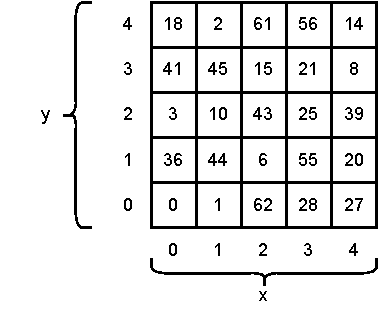
\includegraphics{images/rho.pdf}
    \caption{Rotationsdistanzen der Lanes für $\rho$}
    \label{fig:definition_rho}
\end{figure}
Bei der Rho-Unterfunktion ($\rho$) handelt es sich um eine einfache Bitrotation der einzelnen Lanes.
Bis auf die Lane bei $x=0 und y=0$ werden alle Lanes um eine konstante Distanz nach links rotiert.
Die genauen Distanzen sind in Abb. \ref{fig:definition_rho} aufgeführt.
\begin{align*}
    \rho (\textbf{A}) & \coloneq \textbf{A}^\prime \text{ mit } \\
    \textbf{A}^\prime[x][y] & \coloneq rotl(\textbf{A}[x][y], d[x][y])\ \forall x = 0,...,4;\ y = 0,...,4 \\
    d & :\text{ Eine 5x5 Matrix an Konstanten, siehe Abb. \ref{fig:definition_rho}}
\end{align*}

\subsection{Pi-Unterfunktion}
\begin{figure}
    \center
    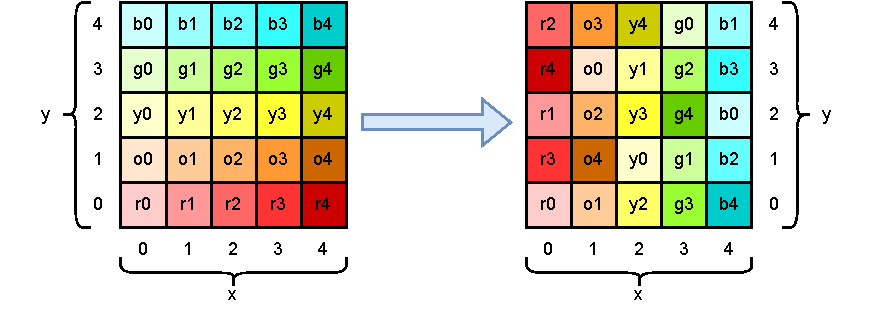
\includegraphics{images/pi.pdf}
    \caption{Visualisierung der $pi$-Permutation}
    \label{fig:definition_pi}
\end{figure}
Di Pi-Unterfunktion ($\pi$) permutiert die Lanes eines State Arrays untereinander nach einer einfachen Vorschrift.
\begin{align*}
    \pi (\textbf{A}) & \coloneq \textbf{A}^\prime \text{ mit } \\
    \textbf{A}^\prime[x][y] & \coloneq \textbf{A}[(x + 3y)\ mod\ 5][x]\ \forall x = 0,...,4;\ y = 0,...,4
\end{align*}

\subsection{Chi-Unterfunktion}

\begin{align*}
    \chi (\textbf{A}) & \coloneq \textbf{A}^\prime \text{ mit } \\
    \textbf{A}^\prime[x][y] & \coloneq \textbf{A}[x][y] \oplus ((\sim \textbf{A}[(x + 1)\ mod\ 5][y]) * \textbf{A}[(x + 2)\ mod\ 5][y])\ & \forall x = & 0,...,4;\\
    && y = & 0,...,4
\end{align*}

\subsection{Iota-Unterfunktion}

\begin{align*}
    \iota (\textbf{A}, r) & \coloneq \textbf{A}^\prime \text{ mit } \\
    \textbf{A}^\prime[x][y] & \coloneq
    \begin{cases}
        \textbf{A}[x][y] \oplus C[r], & x = 0 \text{ und } y = 0 \\
        \textbf{A}[x][y], & \text{sonst}
    \end{cases} \\
    \iota_r (\textbf{A}) & \coloneq \iota(\textbf{A}, r)
\end{align*}

\subsection{KECCAK-p}

\begin{align*}
    \text{keccak-p} (\textbf{A}, r_c) & \coloneq (\iota_r \circ \chi \circ \pi \circ \rho \circ \theta)(\textbf{A}) \\
    \text{keccak-p}_r(\textbf{A}) & \coloneq \text{keccak-p} (\textbf{A}, r)
\end{align*}

\subsection{KECCAK-f}

\begin{align*}
    \text{keccak-f} (\textbf{A}) \coloneq (\bigcomp_{i = 0}^{23} \text{keccak-p}_{i})(\textbf{A})
\end{align*}

\section{Padding-Funktion $pad10^*1$}
Um eine Eingabe beliebiger Länge gescheit verarbeiten zu können, wird eine Padding-Funktion verwendet.
Diese nimmt eine Eingabe beliebiger Länge entgegen und hängt ein einfaches dynamisches Datenmuster an,
sodass die Ausgabelänge ein Vielfaches der gewünschten Blocklänge ist.
SHA-3 verwendet als Padding die Funktion $pad10^*1$. Diese hängt, wie der Name schon vermuten lässt,
zwei 1-Bits an die Ausgabe an und fügt dazwischen so viele Nullen ein, bis die Ausgabe die gewünschte Länge besitzt.

\begin{align*}
	&\begin{alignedat}[t]{2}
	\text{Für} & \text{ eine Eingabe } & M & \in \{0,1\}^*, \\
	& \text{ eine verlangte Blocklänge } & r & \in \mathbb{N} \\
	\end{alignedat} \\
	& \text{ist } pad10^*1(r, M) \coloneq M \mathbin\Vert 1 \mathbin\Vert 0^{(-|M| - 2) mod\ r} \mathbin\Vert 1
\end{align*}

\section{Schwammkonstruktion}
	\begin{figure}
		\center
		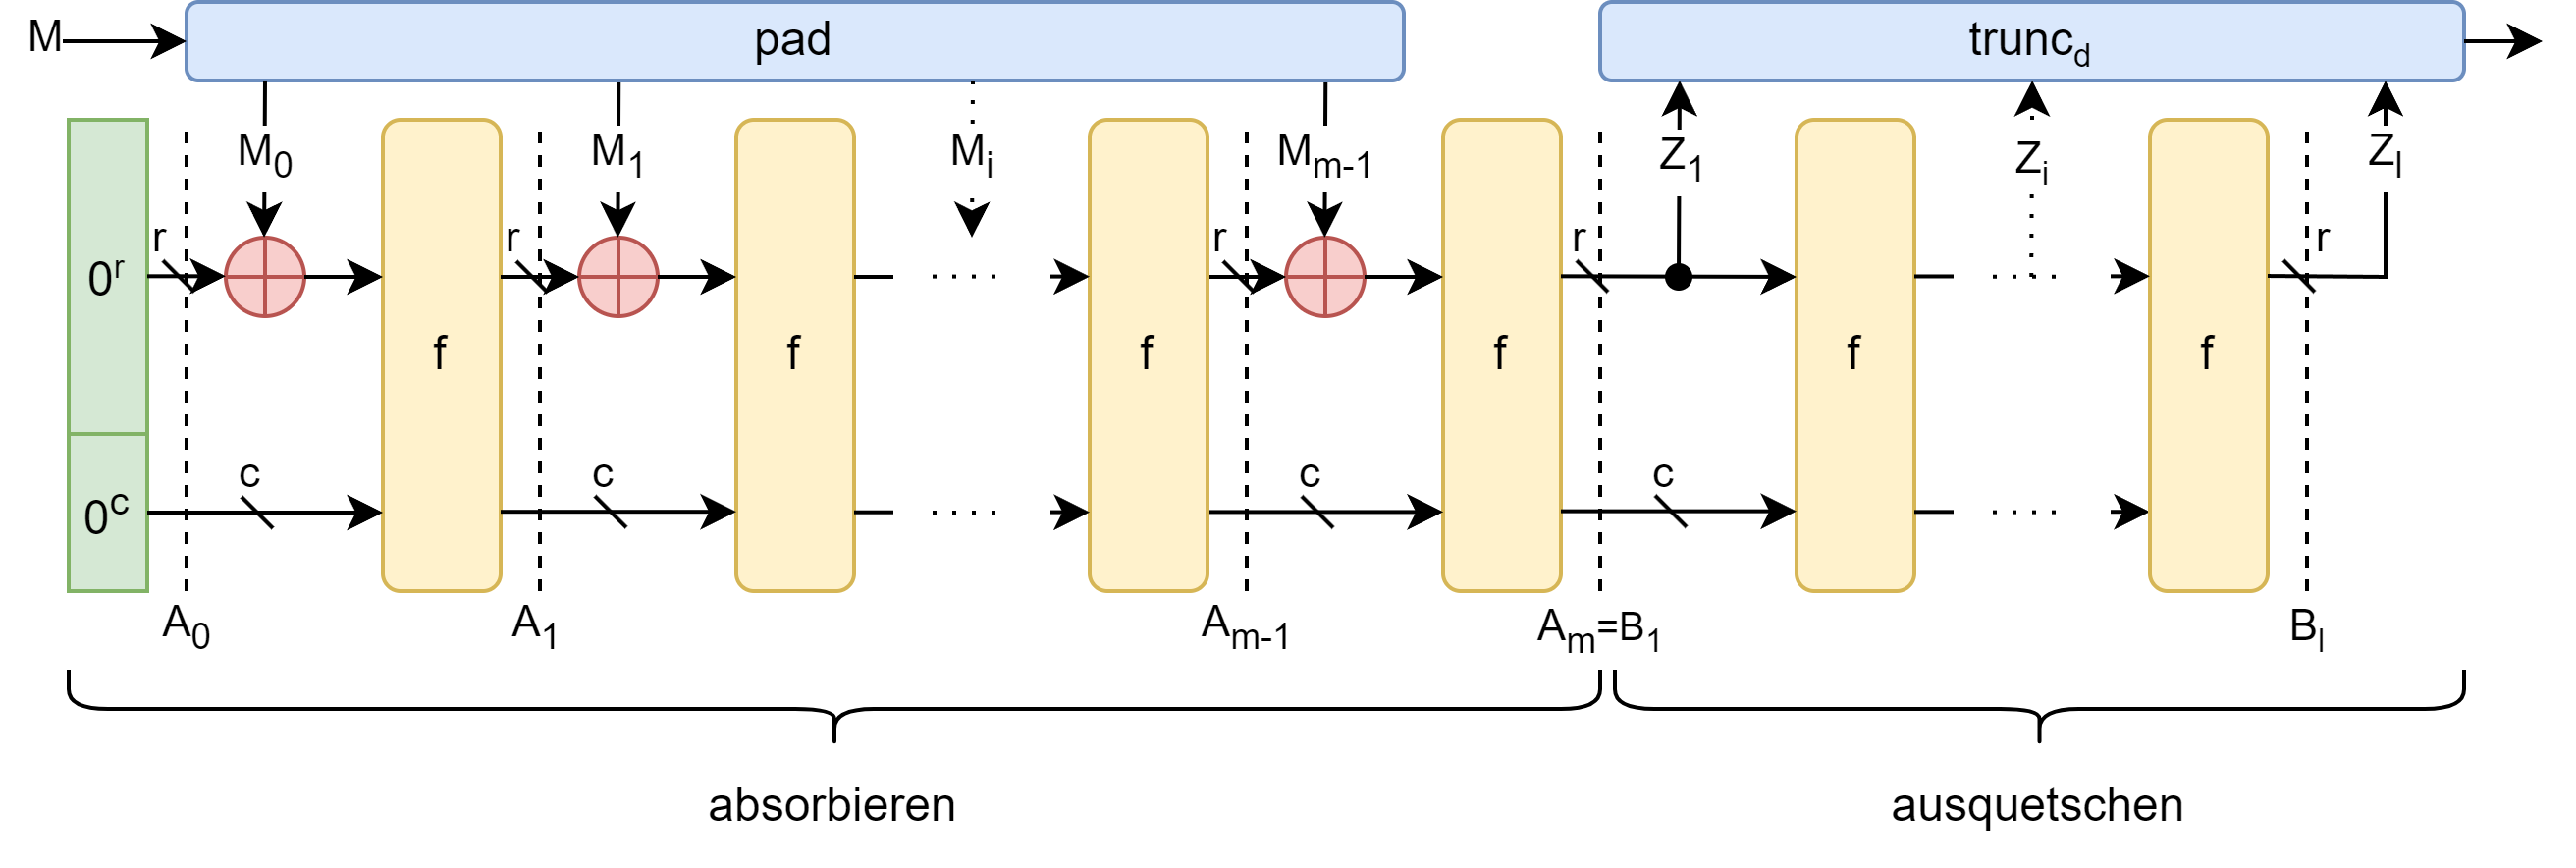
\includegraphics[scale=0.175]{images/Schwammkonstruktion.png}
		\caption{Aufbau der Schwammkonstruktion [Cite missing]}
		\label{fig:schwammkonstruktion}
	\end{figure}
	Um beliebig lange Eingaben zu einem kurzten Hashwert komprimieren zu können, verwendet SHA-3 die sogenannte Schwammkonstruktion.
	Sie erlaubt es eine Eingabe beliebiger Länge auf eine Ausgabe einer beliebigen anderen Länge d abzubilden.
	Dazu wird die Eingabe wie in Abb \ref{fig:schwammkonstruktion} abgebildet erst mit Hilfe einer Padding-Funktion in mehrere gleich große Blöcke einer festgelegten Länge abgebildet.
	Die eingabeblöcke werden dann der Reihe nach vom Schwamm "absorbiert". Danach werden auf ähnliche Weise die Ausgabeblöcke aus dem Schwamm "ausgequetscht".
	Diese Ausgabeblöcke werden dann zur finalen Ausgabe zusammengesetzt. Wenn die Ausgabelänge kein Vielfaches der Blocklänge sein sollte, wird der Rest einfach abgeschnitten.
	Der genaue Definition der Schwammkonstruktion über einer Transformation $f$ mit einer Paddingfunktion $pad$ sieht folgendermaßen aus:
	
	\begin{align*}
		&\begin{alignedat}[t]{2}
			Seien\ & n \in \mathbb{N} && \text{ die Transformationsbreite}, \\
			& r \in \{1,...,n\} && \text{ die Blocklänge}, \\
			& M \in \{0,1\}^* && \text{ die zu verarbeitende Nachricht}, \\
			& m \in \mathbb{N} && \text{ die Anzahl an Blöcken, in die M eingeteilt wird}, \\
			& d \in \mathbb{N} && \text{ die gewünschte Ausgabe}, \\
			& l \coloneq \lceil \frac{d}{r} \rceil && \text{ die benötigte Blockanzahl an Ausgabe}, \\
			& pad: \mathbb{N}x\{0,1\}^* \to (\{0,1\}^r)^+ && \text{ eine Padding-Funktion}, \\
			& f: \{0,1\}^n \to \{0,1\}^n && \text{ eine Transformation}.
		\end{alignedat} \\
		\\
		&\text{Dann ist } SPONGE[f,pad](N,d)\ \text{definiert als:} \\
		&\begin{alignedat}[t]{3}
			SPONGE[f,pad](M, d) & \coloneq \mathbf{Z}[0] \mathbin\Vert ... \mathbin\Vert \mathbf{Z}[d-1]\ mit \\
			M_0...M_{m-1} & \coloneq pad(r, M) \\
			\mathbf{A}_0 & \coloneq 0^n \\
			\mathbf{A}_i & \coloneq f(\mathbf{A}_{i-1} \oplus (M_{i-1} \mathbin\Vert 0^c))\ & \forall i = 1,...,m \\
			\mathbf{B}_1 & \coloneq \mathbf{A}_{m} \\
			\mathbf{B}_i & \coloneq f(\mathbf{B}_{i-1})\ & \forall i = 2,...,l \\
			\mathbf{Z}_i & \coloneq \mathbf{B}_i[0] \mathbin\Vert ... \mathbin\Vert \mathbf{B}_i[r-1] \\
			\mathbf{Z} & \coloneq \mathbf{Z}_1 \mathbin\Vert ... \mathbin\Vert \mathbf{Z}_l
		\end{alignedat}
	\end{align*}

\section{Sicherheitseigenschaften}

\subsection{Kollisionsresistenz}

\subsection{Post-Quantum Sicherheit der Schwammkonstruktion}

\section{Software-Implementierung}